\chapter{Estado da arte}
\label{state}


Neste capítulo, são apresentados os resultados da pesquisa bibliográfica sobre as ferramentas e funcionalidades que poderão estar presentes no sistema a desenvolver. Apresenta-se de forma geral todas as tecnologias possíveis de utilização e respetiva comparação. 






\section{Conceitos tecnológicos}


Nesta secção são apresentados alguns conceitos tecnologias utilizados em toda a dissertação. Com o objetivo de não os repetir, estes serão descritos apenas aqui. 

\begin{itemize}
	\item \ac{HTML}: consiste numa linguagem de marcação que permite estruturar uma página web. 
	\item \ac{CSS}: permite personalizar os componentes existentes \ac{HTML}, isto é, personalizá-los com uma determinada cor, espaçamento ou fonte. 
	\item \ac{JS}: é uma linguagem de programação interpretada. Foi utilizada inicialmente para a criação de aplicações do lado do cliente, sendo que atualmente, já é bastante utilizada do lado do servidor. 
	
	\item Python: é uma  linguagem de programação de alto nível, possuindo os seguintes paradigmas:  orientação a objetos, programação imperativa, programação funcional. 
	
	
	\item \ac{API}: consiste numa interface de programação de aplicações, isto é, disponibiliza um conjunto de funções especificas que permitem ao programador aceder a determinadas funcionalidades.  
	
	\item Web Service: é um tipo de \ac{API} que trabalha com \ac{HTTP},
	ou \ac{SMTP}.
	
	
\end{itemize}



\section{\acl{SGBD}}

Um \acl{SGBD} (\acs{SGBD}) consiste num \textit{software} ou conjunto de \textit{softwares} responsáveis pela manipulação de uma base de dados, permitindo a realização de um conjunto enorme de operações, como por exemplo, operações básicas de manipulação de registos e respectiva visualização, operações estatísticas e respetivos relatórios, automatização de funcionalidades entre outros. Seguidamente são apresentados três \ac{SGBD} e a sua respetiva comparação. 


\subsection{MySQL}


O MySQL é considerado o \ac{SGBD} \textit{open source} mais popular de todo o mundo, sendo líder em aplicações baseadas na web, incluindo o Facebook, Twitter, YouTube, Yahoo! e muitos outros. Está comprovado que possui um elevado desempenho, fiabilidade e facilidade de utilização\cite{MySQL2011}.	






\subsection{SQL Server}

O SQL Server é um \ac{SGBD} desenvolvido pela Microsft com bastante popularidade, tendo suporto para as seguintes linguagens de programação C++, PHP, Java, \ac{JS}, Python entre outras. A ultima versão deste \ac{SGBD} é o SQL Server 2016, estando também disponível para ambiente Linux\cite{linuxsqlserver}.




\subsection{PostgreSQL}

O PostgreSQL é um sistema de gestão de base de dados do tipo objeto-relacional uma vez que permite um modelo de dados orientado a objetos, isto é, possibilita a manipulação de objetos, classes e heranças diretamente no esquemas da base de dados. Segundo o site oficial do PostgreSQL este é considerado um \ac{SGBD} bastante poderoso e com desenvolvimento \textit{open sources}\cite{ThePostgreSQLGlobalDevelopmentGroup2012}. 


%Ele tem mais de 15 anos de desenvolvimento ativo e uma arquitetura comprovada que ela ganhou uma forte reputação de confiabilidade, integridade de dados e correção. Ele roda em todos os principais sistemas operacionais, incluindo Linux, UNIX (AIX, BSD, HP-UX, SGI IRIX, MacOS, Solaris, Tru64), e Windows. É totalmente compatível com ACID, tem suporte completo para chaves estrangeiras, junções views, triggers e procedimentos armazenados (em várias línguas). Ele inclui mais SQL: 2008 tipos de dados, incluindo INTEGER, NUMERIC, BOOLEAN, CHAR, VARCHAR, DATE, INTERVALO e TIMESTAMP. Ele também suporta o armazenamento de grandes objetos binários, incluindo imagens, sons ou vídeo. Ele tem interfaces de programação nativas para C / C ++, Java, .Net, Perl, Python, Ruby, Tcl, ODBC, entre outros, e documentação



\subsection{Comparação e solução adotada}




A tabela \ref{Ranking-engines2016} encontra-se a classifica atribuída pela \textit{Ranking DB-Engines} para os \ac{SGBD} estudados de acordo com a sua popularidade, nos meses de Julho de 2017, Junho de 2017 e Julho de 2016\cite{DB-engines2016}. O MySQL é considerado o mais popular dos estudados, posteriormente o SQL Server e por fim o PostgreSQL. 

Uma vez que o cliente deste sistema pretende que sejam utilizadas tecnologias sem qualquer custo adicional, excluiu-se  desde logo o SQL Server da Microsoft. Restam então duas tecnologias estudadas: PostgreSQL e MySQL. Relatvivamente aos requisitos não funcionais do sistema, estes serão abordados mais à frente nesta dissertação. 



\newpage

\begin{table}[h]
	\centering

	\begin{tabular}{|
			>{\columncolor[HTML]{EFEFEF}}l |l|l|l|}
		\hline
		& \cellcolor[HTML]{EFEFEF}\textbf{Julho 2017} & \cellcolor[HTML]{EFEFEF}\textbf{Junho 2017} & \cellcolor[HTML]{EFEFEF}\textbf{Julho 2016} \\ \hline
		\textbf{MySQL} & 2º lugar & 2º lugar & 2º lugar \\ \hline
		\textbf{SQL Server} & 3º lugar & 3º lugar & 3º lugar \\ \hline
		\textbf{PostgreSQL} & 4º lugar & 4º lugar & 5º lugar \\ \hline
	\end{tabular}
	\caption[\textit{Ranking BD-Engines} para popularidade dos \ac{SGBD} estudados]{\textit{Ranking BD-Engines} para popularidade dos \ac{SGBD} estudados\cite{DB-engines2016}}
	\label{Ranking-engines2016}
\end{table}














Embora as diferenças entre estes os dois SGBD não sejam significativas, podemos também ter em consideração a performance. Para tal, foram realizados alguns estudos que pretendem comparar estas duas ferramentas usando a benchmark TPC-H\footnote{\url{http://www.tpc.org/tpch/}}, expondo que a performance do PostgreSQL é ligeiramente superior à do MySQL na maioria das queries\cite{Lopez2009}. %rever ref.  
A tabela \ref{comp-sqgbdcar} permite comparar algumas das características dos \ac{SGBD} estudados. 




\begin{table}[h]
	\centering

	\begin{tabular}{|
			>{\columncolor[HTML]{EFEFEF}}c |c|c|c|}
		\hline
		& \cellcolor[HTML]{EFEFEF}\textbf{MySQL} & \cellcolor[HTML]{EFEFEF}\textbf{SQL Server} & \cellcolor[HTML]{EFEFEF}\textbf{PostgreSQL} \\ \hline
		\textbf{Modelo} & \multicolumn{3}{c|}{Relacional} \\ \hline
		\textbf{Desenvolvido} & Oracle & Microsoft & \begin{tabular}[c]{@{}c@{}}PostgreSQL\\ Global Development Group\end{tabular} \\ \hline
		\textbf{Lançamento} & 1995 & 1989 & 1989 \\ \hline
		\textbf{Implementação} & C e C++ & C++ & C \\ \hline
		\textbf{Licença} & Open-source & Comercial & Open-source \\ \hline
		\textbf{Versão atual} & \begin{tabular}[c]{@{}c@{}}5.7.18\\ Abril 2017\end{tabular} & \begin{tabular}[c]{@{}c@{}}SQL Server 2016\\ Junho 2016\end{tabular} & \begin{tabular}[c]{@{}c@{}}9.6.3\\ Maio 2017\end{tabular} \\ \hline
		\textbf{Triggers} & \multicolumn{3}{c|}{Suporta} \\ \hline
		\textbf{\begin{tabular}[c]{@{}c@{}}Stored Procedures\\ e Functions\end{tabular}} & \multicolumn{3}{c|}{Suporta} \\ \hline
	\end{tabular}
	\caption{Comparação entre MySQL, SQL Server e PostgreSQL}
	\label{comp-sqgbdcar}
\end{table}



\section{Desenvolvimento web}



No que toca ao desenvolvimento web do sistema, permitindo que este seja adaptado ao cliente/empresa conforme as suas necessidades, poderão ser adotadas duas estratégias distintas: 

\begin{itemize}
	\item Por manipulação local utilizando \ac{JS} que interage com o \ac{DOM}. Exemplo de \textit{frameworks}: Angular.JS, Angular 2, React.JS, Vue.JS
	
	\item Por acesso ao servidor que servirá conteúdos criados em função dos pedidos do cliente. Exemplo de \textit{frameworks}: ASP.net, Django, Flask, Play, Spring
	
\end{itemize}


De modo a facilitar o desenvolvimento do sistema, optou-se que tanto  a nível de \textit{frontend} como de \textit{backend} este seja realizado paralelamente. Posto isto, será utilizada uma framework em que o servidor servirá os conteúdos em função das necessidade do cliente. Esta estratégia é mais eficiente e com tempos de resposta mais curtos, relativamente à primeira apresentada. De seguida, são apresentadas três \textit{frameworks} bastantes populares e com características distintas. 




\subsection{ASP.net}


ASP.net é uma tecnologia de \textit{scripting} que corre do lado do servidor, permitindo colocar numa página web, \textit{scripts} que irão ser executados por um determinado servidor. A sigla \acs{ASP} significa \acl{ASP}. Uma aplicação desenvolvida nesta tecnologia corre num servidor de Internet da Microsft, conhecido por \ac{IIS}, podendo ser desenvolvido recorrendo à linguagem C\# ou Microsoft Visual Basic. Esta tecnologia oferece três modelos para a criação de aplicações web, ASP.NET \textit{Web Forms}, ASP.NET \ac{MVC}, e ASP.NET \textit{Web Pages}, podendo ser criadas aplicações web estáveis e maduras com qualquer um deles\cite{Microsoft2016}. 


\subsection{Flask}


O Flask consiste numa micro-framework desenvolvida em Python baseado nas bibliotecas \ac{WSGI} Werkzeug e Jinja2\footnote{\url{http://jinja.pocoo.org/}}. Esta framework disponibiliza um  modelo simples para desenvolvimento web, um vez que permite economizar bastante tempo na sua conceção. De seguida, são apresentadas algumas das suas principais características\cite{Flask2014}. 


\begin{itemize}
	\item Possui um servidor para desenvolvimento e \textit{degub}
	\item Suporta testes unitários nativamente 
	\item Usa modelos da biblioteca Jinja2
	\item Suporta \textit{cookies} seguros (sessões do lado do cliente)
	\item Compatível com a primeira versão do \ac{WSGI}
	\item Baseado em unicode
	\item Extensa documentação 
\end{itemize}




\subsection{Django}


A framework Django consiste numa ferramenta de desenvolvimento web de alto nível desenvolvida na linguagem Python, possuindo uma arquitetura \ac{MVC}\cite{Deacon2005}, embora com algumas diferenças em relação a esta. No modelo \ac{MVC}, a componente \textit{Model} diz respeito à camada de acesso a dados, a \textit{View} à parte do sistema responsável pela escolha e apresentação da informação e o \textit{Controller} está encarregue de decidir que \textit{views} escolher. Os criadores do Django consideram a sua arquitetura com sendo \ac{MTV}\cite{Index}. 

\begin{itemize}
	\item \textit{Model}: é responsável por manipular, valiar, aceder e relacionar os dados. É considerada a fonte única e definitiva de informação (dados), possuindo os campos essenciais e os comportamentos sobre estes. Geralmente, cada \textit{Model} mapeia uma única tabela na base de dados. 
	
	
	\item \textit{Template}: é responsável pela apresentação dos dados. 

	\item \textit{View}: é responsável pela lógica de negócio e respetiva manipulação, acedendo ao Model e encaminhando o pretendido para o Template. 
	
\end{itemize}



De acordo com as descrições dos autores, esta ferramenta possui as seguintes vantagens\cite{Index}: 


\begin{itemize}
	\item Boa documentação;
	\item Facilidade e rapidez de desenvolvimento e \textit{deployment};
	\item Escalabilidade;
	\item Estabilidade.

\end{itemize}





\subsection{Conclusões e solução adotada}



Uma vez que o cliente do sistema não pretende que existam gasto adicionais, optou-se por utilizar ferramentas \textit{open-source} que permitiu desde logo excluir a tecnologia ASP.net. 


A escolha para desenvolvimento web recaiu sobre o Django uma vez que esta framework recomenda a utilização do PostgreSQL, indicando que permite alcançar um bom equilíbrio entre custo, características, rapidez e estabilidade\cite{Holovaty2009}. 













\newpage
\section{Desenvolvimento mobile}


Uma aplicação móvel, vulgarmente denominada por \textit{app mobile}, consiste num determinado \textit{software} utilizado para realizar funções especificas em dispositivos móveis, como \textit{smartphones} ou \textit{tablets}. Pretende-se que este tipo de \textit{software} permita ao seus utilizadores facilitar o desempenho de determinadas atividades à distância de um simples toque no seu dispositivo. 

No que toca ao desenvolvimento de aplicações móveis, o programador pode recorrer a duas estratégias: desenvolvimento nativo ou multi-plataforma. Esta diferenciação centra-se na forma como o código é produzido, sendo seguidamente apresentadas algumas  vantagens e desvantagens de cada um. 


%A base para esta diferenciação está na forma como o código é desenvolvido para a aplicação móvel. Aplicações nativas são desenvolvidas em específico para cada plataforma (iOS, Android ou Windows), com base no código particular a esse sistema operativo. Aplicações híbridas são apps desenvolvidas com tecnologia web, como é o HTML5, CSS e o JavaScript, que utilizam uma funcionalidade desses sistemas chamada WebView para apresentar o código web como uma aplicação responsiva para qualquer plataforma. Ambas apresentam vantagens e desvantagens, pelo que é essencial estar familiarizado com ambas antes de tomar a sua decisã



\subsection{Plataformas nativas}

Uma aplicação nativa é desenvolvida exclusivamente para ser utilizada por um dispositivo ou plataforma especifica, como é o caso do iOS, Android ou Windows Phone. Nestes casos, são usadas ferramentas e linguagens especificas suportadas pela plataforma, podendo interagir com as funcionalidade do sistema operativo ou aplicações existentes. Seguidamente são apresentadas algumas características de uma plataforma do tipo nativo\cite{Ibm2012a}. 








\begin{itemize}
	\item \textbf{Performance}: acarreta benefícios ao nível da performance, uma vez que as aplicações nativas são desenvolvidas em código especifico e otimizado; 

	
	
	\item \textbf{Desenvolvimento}: tem que ser desenvolvido de raiz para cada dispositivo, exigindo um maior investimento de tempo. 
	
	\item \textbf{Interface}: podem ser utilizadas as funcionalidades da \ac{UI} dos plataformas em questão. 
	
	
	\item \textbf{Recursos disponíveis}: apenas são disponibilizados os recursos de cada plataforma, existindo APIs que permitem o seu acesso. 
	
	

	\item \textbf{\textit{Plug-ins}}: os plug-ins são específicos para cada plataforma, dificultando a sua integração para aplicações multi-plataforma. 
	
	
	\item \textbf{Segurança}: recorre a APIs nativas, utilizando os protocolos de segurança conhecidos da plataforma. 
	
	
\end{itemize}


\subsection{Multi-plataforma}

%http://websocialdev.com/lista-de-frameworks-para-desenvolvimento-mobile/


Uma aplicação multi-plataforma ou híbrida, é desenvolvida utilizando tecnologias web, como por exemplo o \ac{HTML}, \ac{CSS} e \ac{JS}. Este tipo de aplicações utiliza uma funcionalidade denominada por WebView permitindo que o código web seja adaptado a uma aplicação responsiva para uma determinada plataforma. De seguida, são apresentadas algumas características desta estratégia de desenvolvimento\cite{Ibm2012a}. 






% ftp://public.dhe.ibm.com/software/pdf/mobile-enterprise/WSW14182USEN.pdf

\begin{itemize}
	\item \textbf{Performance}: relativamente à performance, não são dados pontos positivos no que toca às aplicações híbridas, uma vez que estas usam  WebViews e outros plug-ins que permitem abstrair o acesso às APIs nativas. 

	
	\item \textbf{Desenvolvimento}: são utilizadas tecnologias web (\ac{HTML}, \ac{CSS} e \ac{JS}), sendo mais eficazes em termos de custo uma vez que permite reutilizar código para diferentes dispositivos. 
	
	
	\item \textbf{Interface}: para aceder à mesma \ac{UI} do sistemas operativos é necessário utilizar plug-ins adicionais. 
	
	
	\item \textbf{Recursos e Plug-ins}: existe muitos recursos disponíveis  para aplicações \linebreak multi-plataforma através de plug-ins, permitindo ter o mesmo efeito em todas as plataforma. Por outro lado, impõe-se a questão da performance. 

	
	\item \textbf{Segurança}: recorrem a plug-ins externos para garantir maior segurança podendo ser potencialmente mais vulneráveis.
	
	
\end{itemize}

Existem enumeras \textit{frameworks} para desenvolvimento multi-plataformas, entre as quais destaco três das mais utilizadas no mercado, Ionic, PhoneGap e Xmarin. 

\begin{itemize}
	\item \textbf{Ionic}: consiste numa ferramenta para desenvolvimento mobile, sendo constituído por outro conjunto de frameworks: Cordova (permite a integração de recursos nativo), AngularJS (criação da \textit{web app}) e Ionic Module e CLI (ferramenta e componentes disponibilizados pelo ionic)\cite{Ionic2016}. 
	
	\item \textbf{PhoneGap}: tal como o Ionic, consiste numa framework mobile que utilizada o Cordava da Apache para aceder aos recursos nativos do sistema. Vantagens desvantagens?? pq é melhor 
	
	\item \textbf{Xmarin}: permite o desenvolvimento mobile a partir do .NET Framework, utilizando C\#, possibilitando que o compilador gere código nativo disponível para qualquer tipo de plataforma. Uma das principais desvantagens do Xmarin prende-se com a necessidade de desenvolver a \ac{UI} para as plataformas necessárias. 
\end{itemize}
 


\subsection{Conclusões e solução adotada}



Um vez que o cliente pretende uma solução mobile multiplataforma, isto é, possível de ser executada em IoS e Android optou-se por utilizar a framework Phonegap. 



Uma das principais desvantagens da utilização deste paradigma multiplataforma é o seu baixo desempenho na utilização de recursos do dispositivo. Uma que não será necessária essa utilização optou-se por utilizar a framework mencionada anteriormente. 



\newpage
\section{REST Frameworks}


Com o evolução da tecnologia, houve a necessidade que os programadores pudessem expor os seus serviços para que possam ser utilizados por outras entidades. Neste sentido, foram criados métodos que permitem a comunicação  entre diferentes sistemas, podendo estes estarem alojados em máquinas ou redes diferentes.   

Para atingir este objetivo, existem atualmente algumas arquiteturas bastante populares, como é o caso do \ac{SOAP} e o \ac{REST}. 


\begin{itemize}
	\item \ac{SOAP}: consiste num protocolo aplicado a ambientes distribuídos e descentralizado. 
	
	formato standard formato obrigado XML
	
	
	\item \ac{REST}: ...
	
	possibilidade de definir o formato das
	mensagens a trocar, sendo normalmente utilizados os formatos JSON ou XML
	
	
\end{itemize}

Dada as vantagens enumeradas relativamente à tecnologia \ac{REST}, optou-se por a utilizar. Seguidamente serão apresentadas algumas frameworks bastante populares no desenvolvimento de APIs REST e a sua respetiva comparação. 



\subsection{Django Rest Framework}


O Django REST Framework é considerado pelos seus autores uma ferramenta poderosa e flexível para a construção de APIs Web \cite{restdjango},



 que pode ser usada juntamente com a framework de desenvolvimento de aplicações Web Django, que quando integrada no desenvolvimento de um determinado \textit{backend} permite a implementação de serviços do tipo REST.



A API navegável Web é uma vitória usabilidade enorme para os desenvolvedores.

Políticas de autenticação , incluindo pacotes para OAuth1a e OAuth2 .

Serialização que suporta tanto ORM e não ORM fontes de dados.

Customizável todo o caminho - basta usar vistas regulares baseadas na função , se você não  precisar dos mais poderosos recursos .

Extensa documentação , e grande apoio da comunidade .

Utilizado e confiável por empresas internacionalmente reconhecidas, incluindo Mozilla , 
Red Hat , Heroku , e Eventbrite .






\subsection{Restlet}



\subsection{Flask-RESTful}


é mais simples e minimalista, permitindo desenvolver serviços REST de
uma forma rápida e leve, possuindo apenas as funcionalidades mais básicas necessárias para o
desenvolvimento deste tipo de serviços.




\subsection{Conclusões e solução adotada}

\ac{HATEOAS}

\begin{table}[h]
	\centering

	\begin{tabular}{|
			>{\columncolor[HTML]{EFEFEF}}l |l|l|l|}
		\hline
		& \cellcolor[HTML]{EFEFEF}\textbf{\begin{tabular}[c]{@{}l@{}}Django Rest\\ Framework\end{tabular}} & \cellcolor[HTML]{EFEFEF}\textbf{Restlet} & \cellcolor[HTML]{EFEFEF}\textbf{Flask-RESTful} \\ \hline
		\textbf{Linguagem} & Python & Java & Python \\ \hline
		\textbf{Serialização} & \begin{tabular}[c]{@{}l@{}}JSON, XML,\\ YAML, HTML\end{tabular} & \begin{tabular}[c]{@{}l@{}}JSON, XML,\\  CSV, YAML\end{tabular} & JSON \\ \hline
		\textbf{Autenticação} & \begin{tabular}[c]{@{}l@{}}Básica, Token, Sessão, \\ OAuth, OAuth2.0\end{tabular} & \begin{tabular}[c]{@{}l@{}}Básica, Digest, \\ AmazonS3, OAuth2.0\end{tabular} & Não \\ \hline
		\textbf{Cache} & Sim & Não & Não \\ \hline
		\textbf{\acs{HATEOAS}} & Sim & Não & Não \\ \hline
		\textbf{Documentação} & \begin{tabular}[c]{@{}l@{}}Intuitiva e simples\\ detalhada e com exemplos\end{tabular} & \begin{tabular}[c]{@{}l@{}}Bastante extensa\\ e detalhada\end{tabular} & \begin{tabular}[c]{@{}l@{}}Detalhada e com \\ alguns exemplos\end{tabular} \\ \hline
	\end{tabular}
		\caption{Comparação entre frameworks REST estudadas.}
		\label{comp-rest}
\end{table}


Django REST Framework é aquela que
apresenta um grau de maturidade maior, apresentando um grande conjunto de funcionalidades
aos programadores, permitindo a utilização de boas práticas de desenvolvimento de serviços
REST, aproveitando todas as vantagens da plataforma Django, nomeadamente o ORM definido
pela própria plataforma, autenticação, gestão de base de dados, de rotas, entre outras.



com autenticação via token 







app mobile
microcontroladores -> controller modulers 


documentação com swager 



\newpage
\section{Microcontroladores}


Um microcontrolador consiste numa solução integrada de um sistema computacional, num único dispositivo físico, sendo uma mistura de \textit{hardware} com \textit{software}. Possui vários módulos principais, um \ac{CPU} onde é realizado todo o processamento, as memórias de instrução e dados (\ac{RAM} e \ac{ROM}) e os portos de entrada e saída (\ac{I/O}), e ainda alguns periféricos (\textit{Timer}, \textit{Serial COM Port}). 

Estes dispositivos são responsáveis pelo processamento de dados, tomada de decisões, controlo do funcionamento de alguns módulos, visualização e conversão da informação recolhida pelos sensores, entre outros. Com o objetivo de simular este sistema, serão utilizados dois microcontroladores bastante comuns no mercado, um Arduino Nano e um Raspberry Pi 3.  


\subsection{Arduino Nano}


Como descrito no site oficial, um Arduino consiste numa plataforma \textit{open-source} de prototipagem eletrónica composta por \textit{hardware} e \textit{software} flexíveis e com elevada facilidade de utilização. Esta plataforma é utilizada para projetos principalmente no contexto do \ac{IoT} e da robótica educativa, sendo possível incorporar vários módulos, dependendo da tarefa que se quer executar\cite{Banzi2012}. 

O Arduino Nano possui um conjunto de pinos que podem ser programados para funcionarem como entradas ou saídas fazendo com que este  microcontrolador interaja com o exterior para os mais diversos fins. Para além dos pinos de \ac{I/O} existem pinos de alimentação que fornecem diversos valores de tensão que podem ser utilizados para transmitir energia elétrica aos diferentes componentes de um projeto\cite{Banzi2012}. Nas figuras \ref{ard2} e \ref{ard1} apresenta-se o Arduino utilizado e a identificação dos diferentes pinos existentes, respectivamente. Adicionalmente, na tabela \ref{caraarduino} encontram-se as principais características desta versão do Arduino.



\begin{figure}[h]
	\centering
	\begin{minipage}[b]{0.49\textwidth}
		\centering
		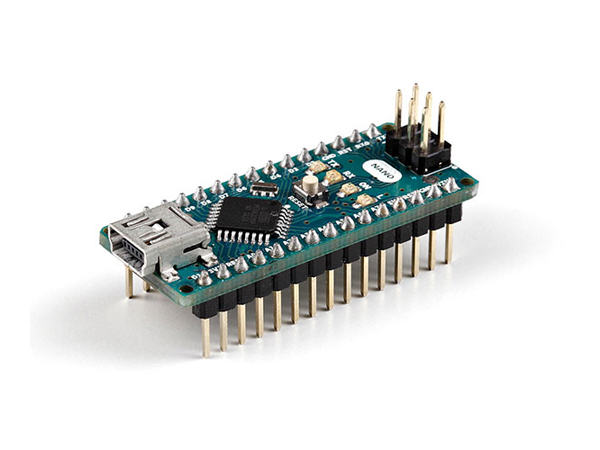
\includegraphics[width=\textwidth]{img/hardware/nano-img.jpg}
		\caption{Arduino Nano}
		\label{ard2}
	\end{minipage}
	\hfill
	\begin{minipage}[b]{0.49\textwidth}
		\centering
		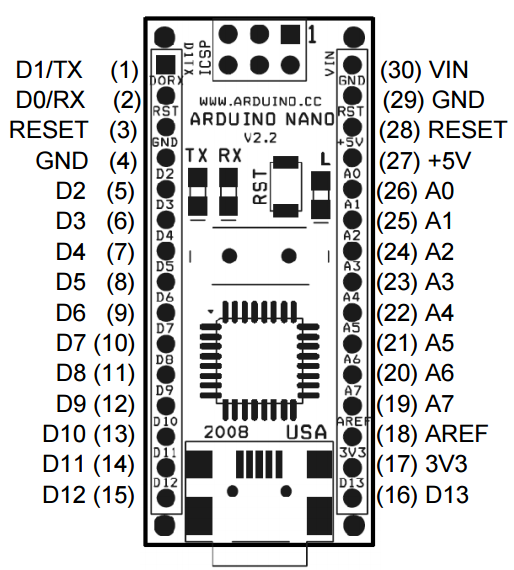
\includegraphics[width=0.6\textwidth]{img/hardware/nano-esquema.png}
		\caption[Identificação dos pinos num Arduino Nano]{Identificação dos pinos num Arduino Nano (Retirado de \cite{arduinonanouser})}
		\label{ard1}
	\end{minipage}
\end{figure}





\newpage

\begin{table}[h]
	\centering
	
	\begin{tabular}{|
			>{\columncolor[HTML]{EFEFEF}}l |l|} \hline
		\textbf{Microcontrolador} & ATmega328 \\ \hline
		\textbf{Tensão de operação} & 5V \\ \hline
		\textbf{Tensão de entrada} & 7-12V \\ \hline
		\textbf{Portas digitais} & 14 (6 podem ser usadas como PWM) \\ \hline
		\textbf{Portas analógicas} & 8 \\ \hline
		\textbf{Corrente nos pinos} \ac{I/O} & 40mA \\ \hline
		\textbf{Memória Flash} & 32KB (2KB usado no bootloader) \\ \hline
		\textbf{Memória \acs{RAM} (SRAM)} & 2KB \\ \hline
		\textbf{EEPROM} & 1KB \\ \hline
		\textbf{Velocidade do \textit{Clock}} & 16MHz \\ \hline
		\textbf{Dimensões} & 45 x 18mm \\ \hline
		\textbf{\ac{LED} interno} & Pino digital 13 \\ \hline
		\textbf{Ligação \ac{USB}} & Ligação ao computador e alimentação \\ \hline
	\end{tabular}
	\caption[Características do Arduino Nano]{Características do Arduino Nano (Adaptado de \cite{Melorose2015})}
	\label{caraarduino}
\end{table}






\subsection{Raspberry Pi 3}

Um Raspberry Pi (figura \ref{rasp1}) é mais poderoso do que outros dispositivos de igual dimensão e incorpora alguns periféricos \ac{I/O}, tal como um computador normal. Tem o tamanho de um cartão de crédito que possui um conjunto de \textit{hardware} integrado que tal como o Arduino, possibilita uma interação com o exterior. Este dispositivo, desenvolvido no Reino Unido pela \textit{Raspberry Pi Foundation}, pode ser ligado a um monitor através da saída HDMI, possuindo também uma saída de áudio e várias portas \ac{USB}. O Raspberry Pi é compatível com sistemas operativos baseados em GNU/Linux, sendo que no trabalho prático desta dissertação será utiliza a versão 3 do Raspberry Pi com a versão Raspbian\footnote{Distribuição Linux oficial do Raspberry Pi:  \url{https://www.raspberrypi.org/downloads/raspbian/}} instalada\cite{RaspberryPiFoundation2012}..

 Na figura \ref{comprasp1} encontram-se os principais componentes da versão utilizada e na tabela \ref{comp23} é feita um comparação entre a versão 2 e 3 do Raspberry Pi, permitindo concluir que a versão utilizada é mais poderosa. 



\begin{figure}[h]
	\centering
	\begin{minipage}[b]{0.49\textwidth}
		\centering
		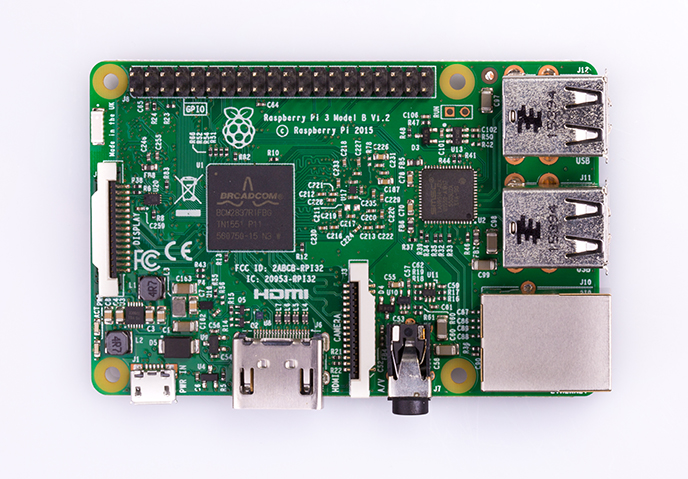
\includegraphics[width=\textwidth]{img/hardware/rasp3-img.jpg}
		\caption{Raspberry Pi 3}
		\label{rasp1}
	\end{minipage}
	\hfill
	\begin{minipage}[b]{0.49\textwidth}
		\centering
		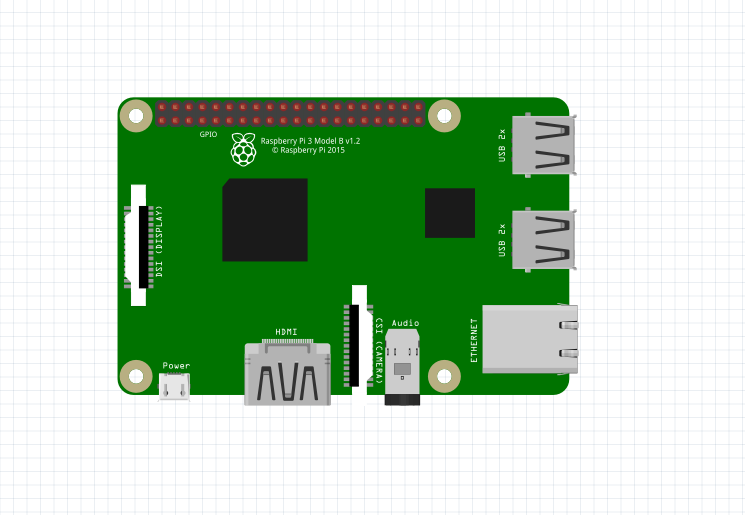
\includegraphics[width=0.8\textwidth]{img/hardware/rasp-esquema.PNG}
		\caption{Principais componentes no Raspberry Pi 3 }
		\label{comprasp1}
		
	\end{minipage}
\end{figure}


\newpage

\begin{table}[h]
	\centering
	\begin{tabular}{|
			>{\columncolor[HTML]{EFEFEF}}l |l|l|}
		\hline
		& \cellcolor[HTML]{EFEFEF}\textbf{Raspberry Pi 2 Model B 1.2} & \cellcolor[HTML]{EFEFEF}\textbf{Raspberry Pi 3 Model B} \\ \hline
		\textbf{CPU} & QUAD Core 900MHz & QUAD Core 1.2GHz \\ \hline
		\textbf{RAM} & 1GB SDRAM & 1GB SDRAM \\ \hline
		\textbf{Potência máxima} & 5V/1.8A & 5V/2.5A \\ \hline
		\textbf{Armazenamento} & MicroSD & MicroSD \\ \hline
		\textbf{USB 2.0} & 4 x Portas USB & 4 x Portas USB \\ \hline
		\textbf{GPIO} & 40 pinos & 40 pinos \\ \hline
		\textbf{Porta Ethernet} & Sim & Sim \\ \hline
		\textbf{Wifi} & Incorporado (versão 802.11n) & Não \\ \hline
		\textbf{Bluetooth LE} & Incorporado (versão 4.1) & Não \\ \hline
	\end{tabular}
	\caption{Comparação entre versão 2 e 3 do Raspberry Pi}
	\label{comp23}
\end{table}









\section{Sensores}


Esta secção tem como objetivo fazer um estudo comparativo entre as diferentes tecnologias usadas para a medição dos vários parâmetros ambientais necessários ao controlo e monitorização da produção de Salicórnia. Serão descritos alguns sensores de temperatura, luminosidade e salinidade existentes no mercado. 



\subsection{Sensor de temperatura }
Existem vários tipos de sensores de temperatura baseados em princípios de funcionamento distintos, nomeadamente os termopares, os termístores e os de circuito integrado. 

\begin{itemize}
	\item \textbf{Termopares}: são sensores de temperatura simples, robustos e de baixo custo, constituídos por duas partes diferentes de material condutor. Podem medir temperaturas entre os -200ºC e os 2315ºC, sendo usados em grande escala\cite{REOTEMPInstrumentCorporation}. 
	 
	
	\item \textbf{Termístor}: são sensores cuja resistência varia com a temperatura, sendo construídos a partir de materiais semicondutores. Um termístor detêm uma maior sensibilidade, pois uma pequena variação de temperatura provoca uma grande variação na sua resistência, permitindo que a temperatura típica seja entre os -100ºC e os 300ºC. Estes sensores são frágeis, baratos e de dimensões reduzidas, sendo suscetíveis a problemas de auto aquecimento\cite{TemperatureSensors}.
	

	\item \textbf{Circuito integrado}: são sensores construídos através de materiais semicondutores, o que possibilita que tenham uma gama de temperatura limitada, geralmente entre os -55ºC e os 150ºC. 	Estão disponíveis com saídas em tensão, ou corrente, linearmente proporcional à temperatura. 


\end{itemize}





\subsection{Sensor de luminosidade }


%O LDR (Light Dependent Resistor) é um componente cuja resistência varia de acordo com a intensidade da luz. Quanto mais luz incidir sobre o componente, menor a resistência. Este sensor de luminosidade pode ser utilizado em projetos com arduino e outros microcontroladores para alarmes, automação residencial, sensores de presença e etc.


Existe uma enorme variedade de sensores de luminosidade/radiação no mercado, contudo para monitorizar a luminosidade incidente numa planta é fundamental conhecer a radiação que é utilizada no processo de fotossíntese, denominada por \ac{PAR}. A figura \ref{grapFoto} ilustra o espectro de absorção de luz pelas plantas. É possível ver que estas são mais sensíveis à luz azul e vermelha (300-700 nm).





\begin{figure}[!htb]
	\centering
	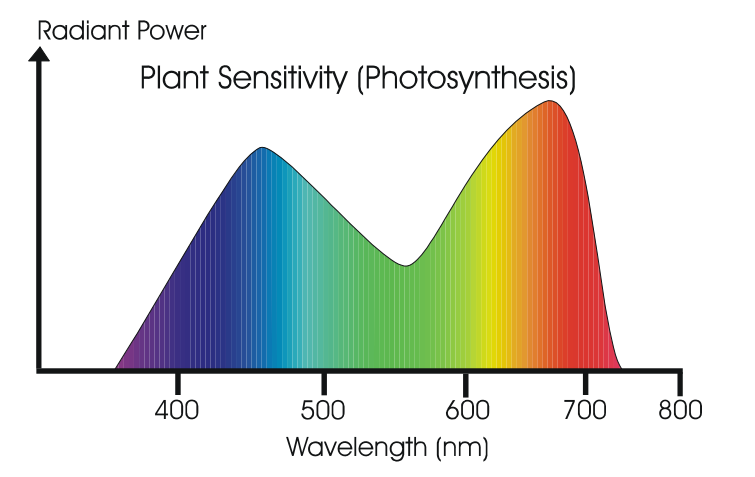
\includegraphics[scale=0.3]{img/plantagrap.png}
	\caption[Sensibilidade luminosa das plantas durante a fotossíntese)]{Sensibilidade luminosa nas plantas durante a fotossíntese (Retirado de \cite{Argus2010})}
	\label{grapFoto}
\end{figure}

Alguns dos sensores de luminosidade/radição mais comuns no mercado são os sensores \ac{PAR}, os piranómetros e os sensores optoelectrónicos, descritos de seguida. 

\begin{itemize}
	\item \textbf{Sensores \ac{PAR}}: são desenhados especificamente para medir a \ac{PAR}, sendo indicados para medir a luz incidente numa planta. Os custos associados a este tipo de sensores são elevados e por isso são utilizados maioritariamente na investigação hortícola. 
	


	
	
	
	\item \textbf{Piranómetros}: estes sensores medem a radiação solar total (radiação ultravioleta, visível e infravermelha), devendo ser utilizados no exterior. Este tipo de sensores é particularmente útil em estações meteorológicas. No entanto, são bastante dispendiosos, podendo ser mais caros dos que os sensores \ac{PAR}. 
	
	
	
	
	\item \textbf{Sensores optoelectrónicos}: são dispositivos eletrónicos que se baseiam em fenómenos fotovoltaicos. Existem três sensores deste tipo, que possuem um elevado desempenho quando afetados pelo ruído e uma elevada sensibilidade. São considerados os sensores de luminosidade mais económicos.  
	 
		\begin{itemize}
			\item \textbf{Fotodíodo}: pode ser visto como um díodo comum, gerando uma corrente ou tensão quando incide radiação sobre ele.
			\item \textbf{Fototransístor}: é um transístor desenhado para receber luz, normalmente num módulo transparente.
			\item \textbf{\ac{LDR}}: trata-se de um material semicondutor cuja resistência diminui com a incidência de luz. Trata-se de um sensor económico e de fácil utilização. 
		\end{itemize}
	
\end{itemize}





\subsection{Sensor de salinidade}


Atualmente ainda não há disponível nenhum sensor que permite medir exatamente a salinidade. Contudo,existem sensores que medem a condutividade elétrica num determinado meio, permitindo concluir o estado do meio relativamente à quantidade de sal existente. 
Um exemplo disso, é o sensor SAL-BTA da Vernier\cite{sall} que permite medir de forma fácil e precisa o teor de sal dissolvido numa solução aquosa.




\section{Tecnologias de comunicação}
\label{state-tecc}
Nesta secção serão apresentadas algumas das tecnologias de comunicação sem fios mais utilizados em \textit{Internet of Things} que permitem a troca de informação entre dispositivos. Serão abordados quatro tecnologias bastante populares comunicação: Zigbee, Bluetooth, Wi-Fi e SigFox. Por fim, é realizada uma comparação entre as tecnologias estudadas. 



\subsection{Zigbee}


Zigbee é um padrão de rede sem fios destinado a aplicações de controlo e sensores remotos, adequado para operações em ambientes isolados. Esta tecnologia é de curto alcance, baixa complexidade e consumo de energia, possuindo ainda uma taxa de dados baixa. Permite uma topologia de rede \textit{mesh} (malha) permitindo elevados níveis de fiabilidade e maior alcance de cobertura, fornecendo mais do que um caminho através da rede para qualquer ligação\cite{Rahman2015}. 	




\subsection{Bluetooth (BLE)}


Bluetooth (BLE) é uma marca característica da versão 4.0 do Bluetooth, sendo projetado para aplicações de baixa potência, utilizada em comunicações de curta distância. Esta tecnologia de comunicação bastante conhecida, consiste numa especificação de rede sem fio de âmbito pessoal, também conhecida por \ac{PANs}, sendo de baixo custo e consumo de energia. O Bluetooth surgiu com a intenção de eliminar o elevado número de cabos existentes na comunicação entre dispositivos, sendo que este padrão funciona na banda de frequência 2,4GHz, conhecida como banda \ac{ISM}\footnote{Faixa de frequência compartilhada por dispositivos, como forno micro-ondas e Wi-Fi}, disponível mundialmente sem a necessidade de licenças\cite{Bruno2002}\cite{BluetoothTM2001}. 


%https://sigarra.up.pt/fcup/en/pub_geral.show_file?pi_gdoc_id=730816




\subsection{Wi-Fi (IEEE 802.11)}


O Wi-Fi é uma tecnologia de recepção de transmissão de dados sem fios, baseado no \textit{standard} IEEE 802.11. Com o evoluir da tecnologia, têm surgido diferentes variações do mesmo \textit{standard}, sendo a variante 802.11g a mais comum. Seguidamente, são apresentadas as característica principais desta variante\cite{Paper2005}\cite{urlwifi}:


\begin{itemize}
	\item Banda de frequência de 2.4 GHz;
	\item Taxa de bits máxima de 54 Mbps na camada física, transferência de dados máxima de 24.7 Mbps;
	\item Topologia em estrela (infraestrutura) e ponto-a-ponto (ad-hoc);
	\item Vários mecanismos de encriptação e autenticação;
\end{itemize}







\subsection{Sigfox}


A tecnologia Sigfox permite a comunicação sem fios entre dispositivos possuindo um baixo consumo de energia, utilizando a banda \ac{ISM}, tal como o Bluetooth. De acordo com o site oficial, o Sigfox é considerado um protocolo leve, permitindo trocas de pequenas mensagens possibilitando um consumo de bateria bastante reduzido\cite{sigfoxsite}. Esta tecnologia é totalmente virada para o \ac{IoT} devido ao seu baixo consumo. 




\subsection{Comparação entre tecnologias de comunicação}

Na tabela \ref{com-tecn} é apresentada uma comparação entre algumas características das tecnologias anteriormente estudadas. 

De acordo com os dados apresentados na tabela, concluímos que o Zigbee e o Sigfox são tecnologias de baixo consumo, contudo o alcance destas é inferior relativamente às tecnologias Bluetooth e Wi-Fi. 




\begin{table}[h]
	\centering

	\begin{tabular}{|
			>{\columncolor[HTML]{EFEFEF}}l |l|l|l|l|}
		\hline
		& \cellcolor[HTML]{EFEFEF}\textbf{Zigbee} & \cellcolor[HTML]{EFEFEF}\textbf{Bluetooth} & \cellcolor[HTML]{EFEFEF}\textbf{Wi-fi} & \cellcolor[HTML]{EFEFEF}\textbf{Sigfox} \\ \hline
		\textbf{IEEE} & 802.15.4 & 802.15.1 & 802.11n & N/A \\ \hline
		\textbf{Banda de frequência} & \begin{tabular}[c]{@{}l@{}}868/915 MHz\\ 2.4 GHz\end{tabular} & 2,4-5,5 GHz & 2,4-5 GHz & \begin{tabular}[c]{@{}l@{}}800 Hz\\ (europa)\end{tabular} \\ \hline
		\textbf{Topologia da rede} & Mesh & Estrela & Estrela & P2P \\ \hline
		\textbf{Energia (consumo)} & Muito baixo & Baixo & Médio & Muito baixo \\ \hline
		\textbf{Alcance} & 10m & aprox. 50m & 100m & \begin{tabular}[c]{@{}l@{}}Rural: 10-15m\\ Urbano: 3-5m\end{tabular} \\ \hline
		\textbf{Bateria (duração)} & Meses-anos & Dias & Horas & 10/15 anos \\ \hline
		
	\end{tabular}
	\caption[Comparação entre tecnologias de comunicação]{Comparação entre tecnologias de comunicação (Adaptado de \cite{Rahman2015})}
	\label{com-tecn}
\end{table}







%\subsection{Módulo bluetooth}







\newpage
%\section{Aplicações relacionadas}



%Seja para comparar, seja para replicar boas funcionalidades, ou seja para conseguir oferecer algo mais ao utilizador final, quando se pretende desenvolver uma determinada aplicação, e importante proceder a uma avaliação de aplicações da mesma área se encontram no mercado. 
%Assim, são aqui abordadas algumas das aplicações relacionadas que são mais utilizadas ou que mais se aproximam daquilo que se pretende para a aplicação a desenvolver neste projeto, tendo em conta os diferentes sistemas operativos.



%\subsection{Multi-monitorização de estufas agrícolas }

%https://repositorio.ipcb.pt/bitstream/10400.11/949/1/Multimonitorizacao%20Estufa%20Agricola.PDF

%\subsection{Agroopar}

%http://www.vidarural.pt/agroopar-os-custos-na-mao-do-agricultor/


%\subsection{outras que vale a pena para comparacao..}

%\subsection{Sistema de Monitorização de Estufas Agrícolas}


%http://www.anje.pt/preview/perfil-coolfarm



%\cite{Abreu2012}


\newpage









